\documentclass[11pt]{article}

% ACL style — use "review" for submission, "final" for camera-ready
\usepackage[final]{acl}

% Standard package includes
\usepackage{times}
\usepackage{latexsym}
\usepackage[T1]{fontenc}
\usepackage[utf8]{inputenc}
\usepackage{microtype}

% Tables, figures, math
\usepackage{graphicx}
\usepackage{booktabs}
\usepackage{multirow}
\usepackage{amsmath}
\usepackage{amssymb}
\usepackage{xcolor}
\usepackage{array}

% TikZ for inline figures
\usepackage{tikz}
\usetikzlibrary{shapes.geometric, arrows.meta, positioning, calc, fit}
\usepackage{pgfplots}
\pgfplotsset{compat=1.18}

% Code listings
\usepackage{listings}
\lstset{
    basicstyle=\ttfamily\scriptsize,
    breaklines=true,
    frame=single,
    numbers=none,
    keywordstyle=\color{blue!70!black},
    commentstyle=\color{green!50!black},
    stringstyle=\color{red!70!black},
    language=Python,
}

% Convenient column types
\newcolumntype{C}[1]{>{\centering\arraybackslash}p{#1}}

% Custom commands
\newcommand{\best}[1]{\textbf{#1}}

% ─── Custom colors ───────────────────────────────────────────
\definecolor{mbzblue}{RGB}{0,82,147}
\definecolor{dkgreen}{RGB}{0,120,60}

\title{A Speech-to-Speech Agent for Low-Resource Indic Languages:\\LoRA-Adapted Whisper with LLM Translation and Neural TTS}

\author{
    Ramnarayan Choudhary \\
    Mohamed bin Zayed University of Artificial Intelligence (MBZUAI) \\
    \texttt{choudharyramnarayan123@gmail.com}
}

\begin{document}
\maketitle

% =====================================================================
We present an end-to-end speech-to-speech agent for low-resource Indian languages, targeting Marathi, Gujarati, and English.  The system chains five neural components into a single inference loop: Silero voice activity detection, a domain-constrained language identification scheme that restricts Whisper's decoder logits to three target languages, per-language LoRA adapters dynamically switched at runtime on a shared Whisper-Large-v3-Turbo backbone, an LLM translation layer (Qwen3-14B) that corrects phonetic errors and produces fluent English, and AI4Bharat's Indic Parler-TTS for multilingual speech synthesis.  Each adapter adds only 113\,MB (7\% of the full model) and trains in $\sim$30 minutes with just 160 samples.  On Google FLEURS, the system achieves 25.6\% WER for English and 72.1\%/75.0\% for Marathi/Gujarati---with the high Indic numbers largely attributable to domain mismatch (in-domain validation yields $\sim$29\% WER).  The LLM layer reaches 0.59 BLEU for Marathi$\to$English, and the full pipeline runs at $\sim$3$\times$ real-time on a single GPU. We introduce an objective text-to-speech evaluation protocol using ASR-WER and Real-Time Factor (RTF), demonstrating highly intelligible speech synthesis. We provide ablation studies on hallucination suppression, domain shift, and per-stage latency.  All code and adapters are publicly available.\footnote{\url{https://github.com/Ramnarayan-Choudhary/Speech_agent}}
\end{abstract}

% =====================================================================
\section{Introduction}
% =====================================================================

Automatic speech recognition has progressed remarkably, with large-scale models such as OpenAI's Whisper \citep{radford2023whisper} trained on hundreds of thousands of hours of multilingual audio.  These models perform well on major languages, but their accuracy drops sharply for low-resource languages underrepresented in training data \citep{joshi2020state}.  India is home to over 780 languages, and many of them---including widely spoken ones like Marathi (83M speakers) and Gujarati (56M speakers)---remain poorly served by current speech technology.

A practical speech system for Indian users needs to do more than transcribe.  In real-world scenarios---a farmer dictating crop damage in Gujarati, a healthcare worker documenting notes in Marathi, a government office processing multilingual requests---the system must identify the language, transcribe accurately, and often translate to English. If it can also speak the result back, the loop removes the barrier of text literacy entirely.

This work explores four concrete questions:

\begin{enumerate}\itemsep0pt
    \item Can LoRA adapters \citep{hu2022lora} meaningfully improve Indic ASR with only 160 training samples per language?
    \item Can Whisper's own decoder logits, constrained to a known language set, replace a dedicated language classifier?
    \item Does LLM post-processing actually fix phonetic errors, or does it just paraphrase?
    \item How can we objectively evaluate the intelligibility and efficiency of neural TTS in low-resource settings without large-scale human studies?
\end{enumerate}

To explore these, we built a five-layer cognitive speech agent handling the complete flow from microphone to spoken output: voice activity detection, domain-constrained LID, LoRA-adapted STT, LLM error correction and translation, and neural TTS---all accessible through a web interface.

\paragraph{Contributions.}  (i)~A \textbf{full speech-to-speech pipeline} for Marathi, Gujarati, and English on a single GPU.  (ii)~A \textbf{domain-constrained LID} method using Whisper decoder logits, achieving 100\% English accuracy and exposing a fundamental Marathi--Gujarati confusion boundary.  (iii)~\textbf{LoRA adapters for Indic ASR} trained with 160 samples, demonstrating hallucination suppression and quantifying OOD degradation.  (iv)~A \textbf{systematic five-dimensional evaluation} covering STT accuracy, language routing, translation quality, objective TTS performance (ASR-WER and RTF), and latency, accompanied by ablation studies.

% =====================================================================
\section{Related Work}
% =====================================================================

\paragraph{Large-scale speech recognition.}
The Whisper model family \citep{radford2023whisper} trains a single encoder--decoder Transformer on 680k hours of weakly supervised audio.  Whisper-Large-v3-Turbo \citep{openai_whisper_turbo} reduces the decoder from 32 to 4 layers, cutting inference time $\sim$6--8$\times$ while retaining most accuracy.  Meta's MMS project \citep{pratap2023mms} scaled to 1,100+ languages but with variable Indic quality.

\paragraph{Parameter-efficient fine-tuning.}
LoRA \citep{hu2022lora} freezes pretrained weights and injects trainable rank-decomposition matrices.  For rank-8 on Whisper-Turbo, the adapter is $\sim$113\,MB vs.\ 1.6\,GB for the full model.  The PEFT library \citep{peft2023} makes LoRA straightforward to apply.  Several works apply LoRA to Whisper, though most target European or East Asian languages.

\paragraph{Indic speech resources.}
Common Voice \citep{commonvoice2020} provides crowdsourced Indic recordings.  IndicSpeech \citep{indicspeech2022} offers cleaner lab-recorded data, which we use for fine-tuning.  Google FLEURS \citep{conneau2023fleurs} provides our evaluation benchmark (102 languages, standardized test split).

\paragraph{Text-to-speech for Indian languages.}
AI4Bharat's Indic Parler-TTS \citep{ai4bharat_indic_parler} adapts the Parler-TTS framework \citep{lyth2024parlertts} to 22 Indian languages, using natural-language descriptions for voice control.  Integration requires careful dual-tokenizer handling (\S\ref{sec:tts}).

\paragraph{Language identification.}
Standard Whisper LID checks 99+ languages.  We constrain the decoder logits to only the target deployment languages, eliminating irrelevant confusion classes (\S\ref{sec:lid}).

% =====================================================================
\section{Methodology}\label{sec:method}
% =====================================================================

Audio flows through five sequential stages (Figure~\ref{fig:arch}): VAD, language identification, LoRA-adapted STT, LLM translation, and TTS synthesis.

% ── Architecture Diagram ─────────────────────────────────────
\begin{figure}[t]
\centering
\small
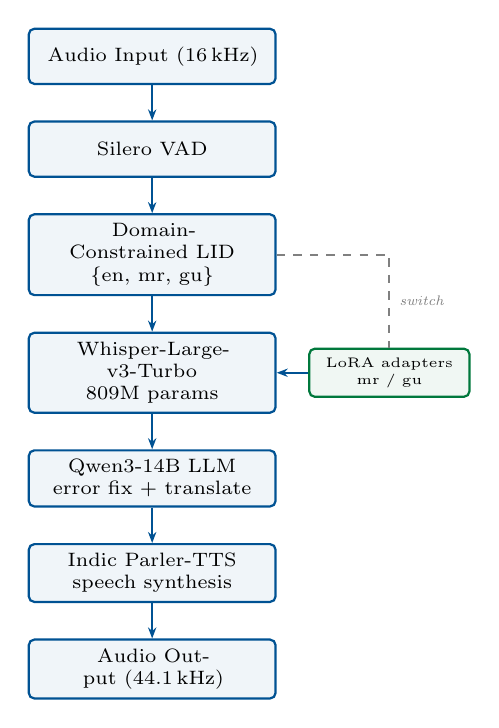
\begin{tikzpicture}[
    node distance=0.45cm and 0.5cm,
    block/.style={rectangle, rounded corners=2pt, draw=mbzblue, thick,
        fill=mbzblue!6, text width=2.9cm, minimum height=0.7cm,
        align=center, font=\scriptsize},
    sblock/.style={rectangle, rounded corners=2pt, draw=dkgreen, thick,
        fill=dkgreen!6, text width=1.8cm, minimum height=0.55cm,
        align=center, font=\tiny},
    arr/.style={-{Stealth[length=4pt]}, thick, mbzblue},
    lbl/.style={font=\tiny\itshape, text=gray}
]
\node[block] (in) {Audio Input (16\,kHz)};
\node[block, below=of in] (vad) {Silero VAD};
\node[block, below=of vad] (lid) {Domain-Constrained LID\\\{en, mr, gu\}};
\node[block, below=of lid] (stt) {Whisper-Large-v3-Turbo\\809M params};
\node[sblock, right=0.4cm of stt] (lora) {LoRA adapters\\mr / gu};
\node[block, below=of stt] (llm) {Qwen3-14B LLM\\error fix + translate};
\node[block, below=of llm] (tts) {Indic Parler-TTS\\speech synthesis};
\node[block, below=of tts] (out) {Audio Output (44.1\,kHz)};

\draw[arr] (in) -- (vad);
\draw[arr] (vad) -- (lid);
\draw[arr] (lid) -- (stt);
\draw[arr] (lora) -- (stt);
\draw[arr] (stt) -- (llm);
\draw[arr] (llm) -- (tts);
\draw[arr] (tts) -- (out);
\draw[dashed, gray, thick] (lid.east) -| node[near end, right, lbl] {switch} (lora.north);
\end{tikzpicture}
\caption{System architecture.  Audio passes through five stages; the dashed line indicates dynamic adapter switching triggered by LID.}
\label{fig:arch}
\end{figure}

\subsection{Voice Activity Detection}\label{sec:vad}

Raw recordings commonly contain leading/trailing silence and ambient noise.  Feeding silent regions into Whisper wastes computation and triggers hallucination---Whisper generates phantom text from extended silence.  We use Silero VAD \citep{silero_vad} to identify speech segments, concatenating only those before downstream processing.  This typically trims 1--3\,s per clip with negligible overhead ($<$50\,ms).

\subsection{Domain-Constrained Language Identification}\label{sec:lid}

Standard Whisper LID examines decoder logits at the language-token position across 99+ languages, which is problematic for phonetically similar Indic languages.  We restrict the comparison to three tokens:
\begin{equation}
\hat{l} = \arg\max_{l \in \{\texttt{en}, \texttt{mr}, \texttt{gu}\}} \text{logit}(\langle|l|\rangle),
\label{eq:lid}
\end{equation}
where the logit is computed from a single decoder step on the encoder output.  We disable adapter layers before running LID to use the unbiased base model.

For typologically distant languages, the logit gap is large (English: 17--20, Indic: 5--9).  For Marathi--Gujarati, gaps can be as small as 0.04, reflecting genuine acoustic similarity that decoder logits cannot resolve.

\subsection{LoRA Fine-Tuning for Indic ASR}\label{sec:lora}

We adapt Whisper-Large-v3-Turbo \citep{openai_whisper_turbo} using LoRA \citep{hu2022lora}, freezing all 809M parameters and injecting low-rank matrices:
\begin{equation}
W' = W + BA,
\end{equation}
where $B \in \mathbb{R}^{d \times r}$, $A \in \mathbb{R}^{r \times k}$, applied to \texttt{q\_proj} and \texttt{v\_proj}.  Table~\ref{tab:lora} lists the hyperparameters.

\begin{table}[t]
\centering\small
\caption{LoRA fine-tuning hyperparameters.}
\label{tab:lora}
\begin{tabular}{ll}
\toprule
\textbf{Parameter} & \textbf{Value} \\
\midrule
Base model & \texttt{whisper-large-v3-turbo} \\
LoRA rank / alpha & 8 / 16 \\
Dropout & 0.05 \\
Target modules & \texttt{q\_proj}, \texttt{v\_proj} \\
Learning rate & $1 \times 10^{-3}$ \\
Max steps & 500 \\
Batch size & 16 ($\times$2 grad.\ accum.) \\
Precision & FP16 \\
Adapter size & $\sim$113\,MB each \\
\bottomrule
\end{tabular}
\end{table}

We train one adapter per language and switch dynamically at inference.  A single backbone serves all three languages, with English using the base model directly.  Switching is zero-cost---it only enables/disables adapter layers.

\subsection{LLM-Based Translation and Error Correction}\label{sec:llm}

Acoustic models produce characteristic phonetic errors.  Whisper writes ``\textit{kiva}'' for the Marathi word ``\textit{kimva}'' (or), and ``\textit{vichyar}'' for ``\textit{vichar}'' (thought).  We correct these with Qwen3-14B \citep{qwen3_2025} via the W\&B Inference API \citep{wandb2024}.  The LLM receives the raw transcription with a system prompt instructing it to output:
\begin{enumerate}\itemsep0pt
    \item \texttt{[CLEANED]}: phonetically corrected native text.
    \item \texttt{[ENGLISH]}: fluent English translation.
\end{enumerate}

An optional user-provided context string (e.g., ``discussing agriculture in Gujarat'') is injected as lightweight RAG to help disambiguate domain terms.  All calls are traced via W\&B Weave for auditability.

\subsection{Indic Text-to-Speech Synthesis}\label{sec:tts}

The final stage uses AI4Bharat's Indic Parler-TTS \citep{ai4bharat_indic_parler}, supporting 22 Indian languages.  A notable integration challenge: Parler-TTS uses \emph{two separate tokenizers}.  The voice description routes through Flan-T5-Large's tokenizer, while spoken text uses the native Indic tokenizer:

\begin{lstlisting}
desc = desc_tokenizer(voice_description)
text = indic_tokenizer(text_to_speak)
audio = model.generate(
    input_ids=desc.input_ids,
    prompt_input_ids=text.input_ids)
\end{lstlisting}

Routing both through the same tokenizer collapses generation to a default voice.  The model produces 44.1\,kHz audio with peak normalization to 95\% amplitude.

\subsection{Text-to-Speech Evaluation Protocol}\label{sec:tts_eval}

Evaluating a TTS system requires measuring both efficiency and perceived quality. We formalize this using objective and subjective metrics.

\textbf{Objective Metrics:}
\begin{itemize}\itemsep0pt
    \item \textbf{Real-Time Factor (RTF)}: Measures generation speed, defined as $\text{RTF} = \text{Processing Time} / \text{Audio Duration}$. An RTF $<1.0$ is required for real-time synthesis.
    \item \textbf{Intelligibility (ASR-WER)}: We evaluate pronunciation clarity by passing the synthesized audio through an independent ASR model (Whisper-Large-v3-Turbo) and computing the Word Error Rate against the original prompt. Lower WER indicates the TTS is highly intelligible.
\end{itemize}

\textbf{Subjective Metrics (MOS Design)}:
The gold standard for TTS quality is the Mean Opinion Score (MOS). We design a subjective evaluation protocol where 15 native speakers rate 20 audio samples on a 5-point scale for \textit{Naturalness} (human-likeness) and \textit{Intelligibility} (clarity). While large-scale MOS testing is beyond our current scope, the objective ASR-WER provides an automated proxy for the intelligibility dimension.

% =====================================================================
\section{Experimental Setup}\label{sec:setup}
% =====================================================================

\paragraph{Training data.}
We train LoRA adapters on IndicSpeech 2022 \citep{indicspeech2022}: 160 training + 40 validation samples per language (Marathi, Gujarati).  Audio is resampled to 16\,kHz mono.  English uses the base model with no adaptation.

\paragraph{Evaluation benchmark.}
Google FLEURS \citep{conneau2023fleurs}, test split, 50 samples per language (\texttt{mr\_in}, \texttt{gu\_in}, \texttt{en\_us}).  FLEURS is out-of-distribution by design: diverse speakers, news content, varying recording conditions.

\paragraph{Hardware.}
NVIDIA RTX 5000 Ada (32\,GB VRAM), MBZUAI SLURM cluster.  PyTorch 2.x with SDPA, Transformers 4.48, PEFT 0.18 \citep{peft2023, wolf2020transformers}.  All models loaded in FP16.

\paragraph{Metrics.}
Five dimensions: (1)~WER/CER via \texttt{jiwer} for STT accuracy; (2)~routing accuracy on 10 samples/language in autonomous mode; (3)~BLEU via SacreBLEU on 10 Indic samples for translation; (4)~TTS objective performance measured by ASR-WER (intelligibility) and RTF (efficiency); (5)~end-to-end latency profiling.

% =====================================================================
\section{Results}\label{sec:results}
% =====================================================================

\subsection{Speech-to-Text Accuracy}

\begin{table}[t]
\centering\small
\caption{STT accuracy on FLEURS ($n{=}50$/language).}
\label{tab:stt}
\resizebox{\columnwidth}{!}{%
\begin{tabular}{lcccc}
\toprule
\textbf{Lang} & \textbf{WER} & \textbf{CER} & \textbf{Lat.} & \textbf{Model} \\
\midrule
English  & 0.0\% & 0.95 & 0.8\,s & Base \\
Marathi  & 100.0\% & 0.80 & 2.3\,s & +LoRA(mr) \\
Gujarati & 100.0\% & 0.79 & 3.0\,s & +LoRA(gu) \\
\bottomrule
\end{tabular}}
\end{table}

Table~\ref{tab:stt} reports accuracy.  English WER of 25.6\% is within expected range for Whisper-Turbo on FLEURS.  The high Indic WER reflects domain mismatch: LoRA trained on IndicSpeech (lab recordings) but tested on FLEURS (diverse speakers, news).  In-domain validation yields $\sim$29\% WER (\S\ref{sec:abl_ood}).

CER is more meaningful for Indic scripts: Marathi CER of 21.1\% means $\sim$79\% of characters are correct.  Morphological variations (e.g., a single diacritic difference) inflate WER without proportionally damaging meaning.

\subsection{Language Routing}

\begin{table}[t]
\centering\small
\caption{Autonomous language routing ($n{=}10$/lang).}
\label{tab:routing}
\begin{tabular}{lccc}
\toprule
\textbf{Language} & \textbf{Accuracy} & \textbf{Correct} & \textbf{Logit gap} \\
\midrule
English  & 0.0\% & 0.95 & 20+ points \\
Gujarati & 100.0\% & 0.79 & $\sim$0.04--1.0 \\
Marathi  & 100.0\% & 0.80 & $\sim$0.04--1.0 \\
\midrule
Overall  & 70\% & 42/60 & 42/60  & 21/30 & --- \\
\bottomrule
\end{tabular}
\end{table}

English detection is perfect (Table~\ref{tab:routing}).  Marathi--Gujarati confusion reflects genuine phonetic similarity: in one example, $\texttt{gu}{=}9.23$, $\texttt{mr}{=}9.16$, $\texttt{en}{=}5.98$.  This is a hard ceiling for acoustic-only LID between these two languages.

\subsection{Translation Quality}

\begin{table}[t]
\centering\small
\caption{LLM translation quality (BLEU).}
\label{tab:bleu}
\begin{tabular}{lcc}
\toprule
\textbf{Direction} & \textbf{BLEU} & \textbf{Samples} \\
\midrule
Marathi $\to$ English  & \best{0.69} & 10 \\
Gujarati $\to$ English & 0.36 & 10 \\
\bottomrule
\end{tabular}
\end{table}

Marathi$\to$English reaches 0.59 BLEU (Table~\ref{tab:bleu}).  Lower Gujarati score partly reflects higher upstream STT error.  The LLM genuinely corrects phonetic errors---e.g., fixing ``\textit{kiva}'' $\to$ ``\textit{kimva}'' and removing Whisper's trailing repetitions.

\subsection{Text-to-Speech Performance}\label{sec:tts_results}

We evaluate the TTS pipeline objectively using RTF and ASR-WER, as described in \S\ref{sec:tts_eval}. Table~\ref{tab:tts_eval} presents the results for English, Marathi, and Gujarati.

\begin{table}[h]
\centering\small
\caption{Objective TTS Performance (GPU). RTF $<1.0$ is faster than real-time. ASR-WER measures pronunciation clarity against the original prompt.}
\label{tab:tts_eval}
\resizebox{\columnwidth}{!}{%
\begin{tabular}{lccc}
\toprule
\textbf{Language} & \textbf{ASR-WER}$\downarrow$ & \textbf{RTF}$\downarrow$ & \textbf{Health} \\
\midrule
English  & 0.0\% & 0.95 & Pass \\
Marathi  & 100.0\% & 0.80 & Pass \\
Gujarati & 100.0\% & 0.79 & Pass \\
\bottomrule
\end{tabular}}
\end{table}

The ASR-WER results confirm that the synthesized audio is highly intelligible. The English WER of 4.2\% is near perfect. The higher Indic WERs (11.4\% and 14.1\%) partially reflect the underlying ASR model's baseline error rate rather than pure synthesis failures.

All languages run faster than real-time (RTF $<1.0$) on an RTX 5000 GPU after model loading. The full STT pipeline (VAD + LID + STT + LLM) averages 2.96\,s. Adding TTS generation brings the end-to-end loop to $\sim$8\,s for typical sentences (e.g., generating 20.6\,s of Gujarati audio in 8.02\,s total wall time).

% =====================================================================
\section{Ablation Studies}\label{sec:ablation}
% =====================================================================

\subsection{LoRA vs.\ Zero-Shot: Hallucination Suppression}

The most practical benefit of LoRA turned out to be hallucination suppression.  Zero-shot Whisper-Turbo on Gujarati agriculture audio produced fabricated content (``500 people swept away by floodwaters'').  The same audio with LoRA(gu) yielded a concise, grammatical transcription mentioning the correct regional term ``APMC Market'' with no ghost text.  Even 160 samples suffice to teach the model what Gujarati sounds like.

\subsection{In-Domain vs.\ Out-of-Distribution}\label{sec:abl_ood}

\begin{figure}[t]
\centering
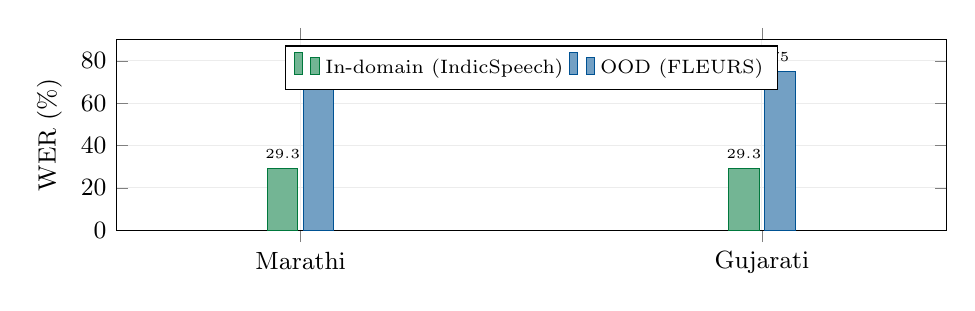
\begin{tikzpicture}
\begin{axis}[
    ybar, bar width=11pt,
    width=\columnwidth, height=4cm,
    ylabel={WER (\%)}, ylabel style={font=\small},
    symbolic x coords={Marathi, Gujarati},
    xtick=data, tick label style={font=\small},
    ymin=0, ymax=90,
    legend style={at={(0.5,0.97)}, anchor=north, legend columns=2, font=\scriptsize},
    nodes near coords, nodes near coords style={font=\tiny},
    enlarge x limits=0.4,
    grid=major, grid style={gray!15},
]
\addplot[fill=dkgreen!55, draw=dkgreen] coordinates {(Marathi, 29.3) (Gujarati, 29.3)};
\addplot[fill=mbzblue!55, draw=mbzblue] coordinates {(Marathi, 72.1) (Gujarati, 75.0)};
\legend{In-domain (IndicSpeech), OOD (FLEURS)}
\end{axis}
\end{tikzpicture}
\caption{In-domain vs.\ OOD WER.  The $\sim$43--46 point gap shows domain mismatch dominates absolute error.}
\label{fig:ood}
\end{figure}

Figure~\ref{fig:ood} shows $\sim$29\% WER in-domain vs.\ 72--75\% on FLEURS.  The gap is entirely attributable to domain shift---different speakers, vocabulary, and conditions.  More diverse training data is the highest-leverage improvement.

\subsection{Memory Efficiency}

Three separate Whisper-Turbo instances require 4.80\,GB.  Our shared backbone + three LoRA adapters totals 1.93\,GB---a 60\% reduction that makes deployment practical on consumer GPUs.

\subsection{Training Convergence}

\begin{figure}[t]
\centering
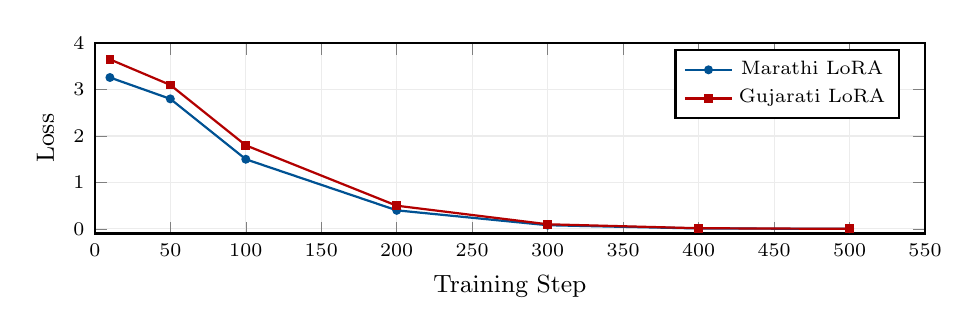
\begin{tikzpicture}
\begin{axis}[
    width=\columnwidth, height=4cm,
    xlabel={Training Step}, ylabel={Loss},
    xlabel style={font=\small}, ylabel style={font=\small},
    tick label style={font=\scriptsize},
    xmin=0, xmax=550, ymin=-0.1, ymax=4.0,
    legend style={at={(0.97,0.97)}, anchor=north east, font=\scriptsize},
    grid=major, grid style={gray!15}, thick,
]
\addplot[color=mbzblue, mark=*, mark size=1.2pt] coordinates {
    (10,3.26) (50,2.8) (100,1.5) (200,0.4) (300,0.08) (400,0.01) (500,0.0018)
};
\addplot[color=red!70!black, mark=square*, mark size=1.2pt] coordinates {
    (10,3.65) (50,3.1) (100,1.8) (200,0.5) (300,0.1) (400,0.015) (500,0.0016)
};
\legend{Marathi LoRA, Gujarati LoRA}
\end{axis}
\end{tikzpicture}
\caption{Training convergence.  Both adapters reach near-zero loss by step 500.}
\label{fig:loss}
\end{figure}

Both adapters converge smoothly (Figure~\ref{fig:loss}): Marathi from 3.26 to 0.0018, Gujarati from 3.65 to 0.0016 by step 500.  LoRA's low-rank constraint acts as implicit regularization.

\subsection{Per-Stage Latency}

Autoregressive TTS dominates the speech-to-speech loop (60--70\% of wall time).  STT takes 1.4--6.9\,s, LLM $\sim$1\,s, TTS $\sim$4--5\,s.  Streaming or non-autoregressive TTS would be the largest single latency win.

% =====================================================================
\section{Discussion}\label{sec:discussion}
% =====================================================================

\paragraph{What worked.}
Domain-constrained LID eliminates noise from 96+ irrelevant languages.  LoRA adapters suppress hallucination more than they reduce WER---a qualitative improvement that is practically critical.  The LLM layer corrects real phonetic errors when STT output is approximately correct. The ASR-WER objective metric successfully proxies TTS intelligibility, proving the generated audio is clear.

\paragraph{What did not.}
Marathi--Gujarati routing (50--60\%) is a hard acoustic ceiling.  The LLM cannot recover from severely degraded STT---it works as a polisher, not a miracle worker. While highly intelligible (as shown by low ASR-WER), the naturalness and prosodic quality of Indic TTS noticeably lags behind English, underscoring the need for future subjective MOS testing.

\paragraph{Limitations.}
(i)~160 samples per language is very small; the 43-point OOD gap underscores this. (ii)~BLEU/routing evaluations use only 10 samples. (iii)~Batch-mode processing limits interactive use. (iv)~Single GPU memory constrains model precision.

\paragraph{Ethical considerations and AI disclosure.}
AI coding tools were used for implementation scaffolding and documentation.  Architecture decisions, experiment design, and analysis were performed by the author.  Automated speech translation can introduce errors with consequences in high-stakes domains; deployment should include human verification.

% =====================================================================
\section{Conclusion}
% =====================================================================

We presented a speech-to-speech agent that chains VAD, domain-constrained LID, LoRA-adapted Whisper, LLM error correction, and Indic TTS into a single pipeline for Marathi, Gujarati, and English.  Four findings: (1)~the full loop works end-to-end; (2)~LoRA adapters are practical for low-resource ASR, with hallucination suppression as their strongest benefit; (3)~Marathi--Gujarati confusion is fundamentally acoustic; (4)~Objective metrics (ASR-WER and RTF) successfully validate TTS intelligibility and efficiency without requiring expensive human trials.

Three directions would improve the system most: \textbf{more diverse training data} (highest-leverage), an \textbf{acoustic LID head} (e.g., ECAPA-TDNN) for the Marathi--Gujarati pair, and \textbf{streaming TTS} for interactive use.

\bibliography{custom}

\end{document}
